% This file was created with tikzplotlib v0.10.1.
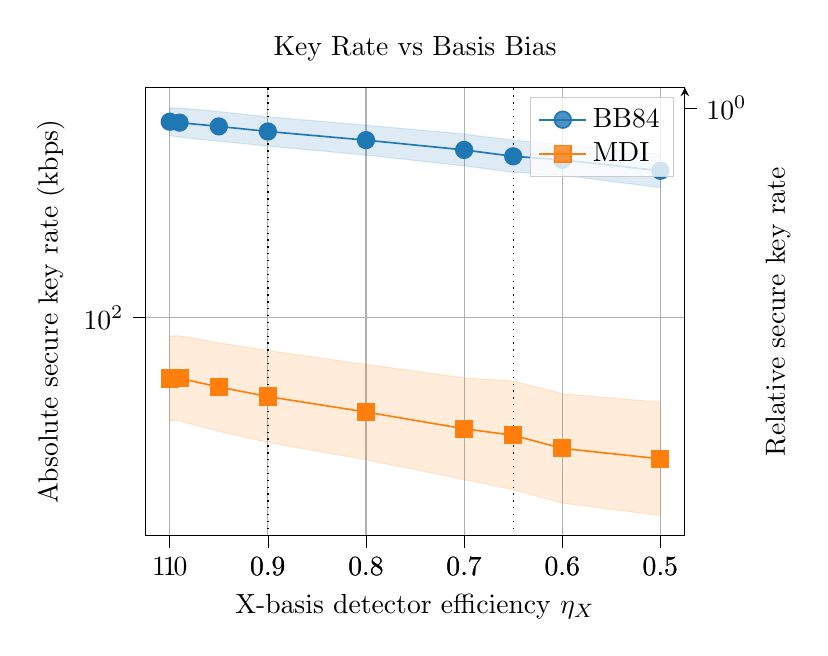
\begin{tikzpicture}

\definecolor{darkgray176}{RGB}{176,176,176}
\definecolor{darkorange25512714}{RGB}{255,127,14}
\definecolor{darkred}{RGB}{139,0,0}
\definecolor{dimgray}{RGB}{105,105,105}
\definecolor{lightgray204}{RGB}{204,204,204}
\definecolor{steelblue31119180}{RGB}{31,119,180}

\begin{axis}[
legend cell align={left},
legend style={fill opacity=0.8, draw opacity=1, text opacity=1, draw=lightgray204},
log basis y={10},
tick align=outside,
tick pos=left,
x dir=reverse,
x grid style={darkgray176},
xlabel={X-basis detector efficiency \(\displaystyle \eta_X\)},
xmajorgrids,
xmin=0.475, xmax=1.025,
xtick style={color=black},
xtick={0.4,0.5,0.6,0.7,0.8,0.9,1,1.1},
xticklabels={
  \(\displaystyle {0.4}\),
  \(\displaystyle {0.5}\),
  \(\displaystyle {0.6}\),
  \(\displaystyle {0.7}\),
  \(\displaystyle {0.8}\),
  \(\displaystyle {0.9}\),
  \(\displaystyle {1.0}\),
  \(\displaystyle {1.1}\)
},
y grid style={darkgray176},
ylabel={Absolute secure key rate (kbps)},
ymajorgrids,
ymin=25.5957294486317, ymax=421.359660424859,
ymode=log,
ytick style={color=black},
ytick={1,10,100,1000,10000},
yticklabels={
  \(\displaystyle {10^{0}}\),
  \(\displaystyle {10^{1}}\),
  \(\displaystyle {10^{2}}\),
  \(\displaystyle {10^{3}}\),
  \(\displaystyle {10^{4}}\)
}
]
\path [draw=red, fill=red, opacity=0.08]
(axis cs:0.65,0)
--(axis cs:0.65,1)
--(axis cs:0.9,1)
--(axis cs:0.9,0)
--cycle;
\path [draw=steelblue31119180, fill=steelblue31119180, opacity=0.15]
(axis cs:1,370.986548062277)
--(axis cs:1,312.221757160205)
--(axis cs:0.99,308.939296569378)
--(axis cs:0.95,301.364311242892)
--(axis cs:0.9,292.308264812931)
--(axis cs:0.8,276.365988648629)
--(axis cs:0.7,258.359901126666)
--(axis cs:0.65,248.130563506323)
--(axis cs:0.6,243.753464795195)
--(axis cs:0.5,225.51095938363)
--(axis cs:0.5,278.352083407026)
--(axis cs:0.5,278.352083407026)
--(axis cs:0.6,295.204854610271)
--(axis cs:0.65,303.158565228516)
--(axis cs:0.7,315.180835312702)
--(axis cs:0.8,333.039576969088)
--(axis cs:0.9,350.844656698041)
--(axis cs:0.95,362.614122297038)
--(axis cs:0.99,370.770153724442)
--(axis cs:1,370.986548062277)
--cycle;

\path [draw=darkorange25512714, fill=darkorange25512714, opacity=0.15]
(axis cs:1,89.1159992916538)
--(axis cs:1,52.4652455094078)
--(axis cs:0.99,52.5321904893955)
--(axis cs:0.95,49.2067999931605)
--(axis cs:0.9,45.8972672172373)
--(axis cs:0.8,41.1838372370318)
--(axis cs:0.7,36.3848593653395)
--(axis cs:0.65,34.1700936990252)
--(axis cs:0.6,31.4206558195427)
--(axis cs:0.5,29.0711561514397)
--(axis cs:0.5,58.9958381032021)
--(axis cs:0.5,58.9958381032021)
--(axis cs:0.6,62.2459676994748)
--(axis cs:0.65,67.3937908062584)
--(axis cs:0.7,68.6718290726371)
--(axis cs:0.8,74.7774855330351)
--(axis cs:0.9,81.4220801547266)
--(axis cs:0.95,85.5690470925568)
--(axis cs:0.99,89.3702736573373)
--(axis cs:1,89.1159992916538)
--cycle;

\addplot [semithick, steelblue31119180, mark=*, mark size=3, mark options={solid}]
table {%
1 340.338172879274
0.99 338.445668432245
0.95 330.573675922619
0.9 320.241772444341
0.8 303.382286806899
0.7 285.359579212631
0.65 274.267944940564
0.6 268.248403789502
0.5 250.542302566953
};
\addlegendentry{BB84}
\addplot [semithick, darkorange25512714, mark=square*, mark size=3, mark options={solid}]
table {%
1 68.3775751372687
0.99 68.518729117349
0.95 64.8889743014079
0.9 61.1314237544391
0.8 55.4943582104255
0.7 49.9861465124942
0.65 47.9880417039741
0.6 44.2245308311979
0.5 41.4134908186118
};
\addlegendentry{MDI}
\addplot [line width=0.48pt, black, dotted, forget plot]
table {%
0.65 25.5957294486317
0.65 421.359660424859
};
\addplot [line width=0.48pt, black, dotted, forget plot]
table {%
0.9 25.5957294486317
0.9 421.359660424859
};
\draw (axis cs:0.6434,0.01) node[
  scale=0.35,
  anchor=south west,
  text=dimgray,
  rotate=0.0
]{0.65};
\draw (axis cs:0.775,0.97) node[
  scale=0.35,
  anchor=north,
  text=darkred,
  rotate=0.0
]{\itshape Realistic hardware regime};
\end{axis}

\begin{axis}[
axis y line=right,
log basis y={10},
tick align=outside,
title={Key Rate vs Basis Bias},
x dir=reverse,
x grid style={darkgray176},
xmin=0.475, xmax=1.025,
xtick pos=left,
xtick style={color=black},
y grid style={darkgray176},
ylabel={Relative secure key rate},
ymin=0.109519823530306, ymax=1.11106237569794,
ymode=log,
ytick pos=right,
ytick style={color=black},
ytick={0.01,0.1,1,10,100},
yticklabel style={anchor=west},
yticklabels={
  \(\displaystyle {10^{-2}}\),
  \(\displaystyle {10^{-1}}\),
  \(\displaystyle {10^{0}}\),
  \(\displaystyle {10^{1}}\),
  \(\displaystyle {10^{2}}\)
}
]
\addplot [semithick, steelblue31119180, opacity=0, mark=*, mark size=3, mark options={solid}]
table {%
1 1
0.99 0.99443934122635
0.95 0.971309427696436
0.9 0.940951670907446
0.8 0.891414219687062
0.7 0.838458926891678
0.65 0.805868888054038
0.6 0.788181947150123
0.5 0.7361569242949
};
\addplot [semithick, darkorange25512714, opacity=0, mark=square*, mark size=3, mark options={solid}]
table {%
1 0.200910684096326
0.99 0.201325430343819
0.95 0.19066028871356
0.9 0.179619650764605
0.8 0.163056520345458
0.7 0.146871995255805
0.65 0.141001055796925
0.6 0.129942904896787
0.5 0.121683355317601
};
\end{axis}

\end{tikzpicture}
